\documentclass{beamer}
\usepackage{beamerthemeshadow}
\usepackage{color}
\usepackage[all]{xy}

%% Elena's favorite green (thanks, Fernando!)
\definecolor{ForestGreen}{RGB}{34,139,34}
\definecolor{BlueViolet}{RGB}{138,43,226}
\definecolor{Coquelicot}{RGB}{255, 56, 0}
\definecolor{Teal}{RGB}{2,132,130}
%Uncomment this if you want to show work-in-progress comments
\newcommand{\comment}[1]{{\bf \tt  {#1}}}
% Uncomment this if you don't want to show comments
%\newcommand{\comment}[1]{}
% for color names see https://www.overleaf.com/learn/latex/Using_colors_in_LaTeX
\newcommand{\emcomment}[1]{\textcolor{ForestGreen}{\comment{Elena: {#1}}}}
\newcommand{\todo}[1]{\textcolor{blue}{\comment{To Do: {#1}}}}
\newcommand{\tkcomment}[1]{\textcolor{Teal}{\comment{Tristan: {#1}}}}
\newcommand{\jscomment}[1]{\textcolor{olive}{\comment{Jaydon: {#1}}}}
\newcommand{\jwcomment}[1]{\textcolor{violet}{\comment{John: {#1}}}}
%%%%%%%%%%%%%%%%%%%%%%%%%%%%%%%%%%%%%%%%%%


%%%% choose your presentation style:
\mode<presentation>
{
  \usetheme{Copenhagen} %%%
 \usecolortheme{beaver}

%%% set style for ovelays: lists (and other text) appearing one item at a time
%%% This will create a dimmed preview of next item:
\setbeamercovered{transparent}
%%% This will hide it entirely:
%\setbeamercovered{invisible}
}
%% if you don't want page numbers to show: 
\setbeamertemplate{footline}[page number]{}

%%%% 25 minutes time slot, including questions 

\begin{document}
\title{A beginner-friendly environment for exploring error messages in the Clojure programming language.}
\author{Tristan Kalvoda, Elena Machkasova, Jaydon Stanislowski, and John Walbran}
\institute[UMN Morris] % (optional, but mostly needed)
{
 % \inst{1}%
  University of Minnesota, Morris
}
\date[]  
{Midwest Instruction and Computing Symposium, April 2025}

\begin{frame}
  \titlepage
\end{frame}

\begin{frame}

  \frametitle{Outline}
\tableofcontents
\end{frame}

\section{Overview of Clojure and Its Error Messages}

\subsection{Clojure language and Syntax}
\begin{frame}
\frametitle{Clojure Language and Syntax}
What is Clojure? - Clojure language and Syntax
\begin{itemize}
  \item Clojure is a part of the Lisp language family
  \item Syntax
  \begin{itemize}
    \item prefix notation (operators before operands).
    \item expressions are surrounded by parentheses.
  \end{itemize}
\end{itemize}
Example: \texttt{(/ 9 3)} denotes 9 divided by 3
\end{frame}

\begin{frame}
  \frametitle{Clojure Language and Syntax}
  \begin{itemize}
    \item Clojure is implemented in Java and runs on the Java Virtual Machine (JVM)
    % \begin{itemize}
      % \item executed code compiles to JVM bytecode \emcomment{I corrected the line below slightly. Not sure if you need this line.}
    % \end{itemize}
    \item Clojure code \(\rightarrow\) Java code \(\rightarrow\) JVM bytecode \(\rightarrow\) \\ executed on JVM
  \end{itemize}
\end{frame}

\begin{frame}
  \frametitle{Clojure Language and Syntax}
  Clojure's REPL
  \begin{itemize}
    \item interactive environment for code evaluation
    \item Read \(\rightarrow\) Evaluate \(\rightarrow\) Print \(\rightarrow\) Loop
  \end{itemize}
  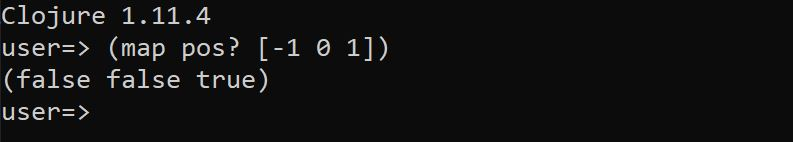
\includegraphics{../resources/cljScreenshot.JPG}  
\end{frame}

\subsection{Clojure's Error Messages}
\begin{frame}
  \frametitle{Clojure's Error Messages}
  Clojure Exceptions
  \begin{itemize}
    \item an event or error that disrupts the normal flow of a program's execution
    \item Clojure syntax errors will also result in a Java exception %\emcomment{mention that it is a Java exception}
  \end{itemize}
  Error Messages
  \begin{itemize}
    \item generate when a exception occurs
    \item provide error type, cause, and location
  \end{itemize}
\end{frame}

\begin{frame}
    \frametitle{Clojure's Error Messages}
    Anatomy of a Clojure Error Message \\
    \texttt{=> (/ 9 0)} \\
    \texttt{Execution error (ArithmeticException) at user/eval1 (REPL:1).} \\
    \texttt{Divide by zero}
    \begin{itemize}
      \item \texttt{ArithmeticException}: The type of error that occurred.
      \item \texttt{user/eval1 (REPL:1)}: The location where the error happened (in this case, REPL, line 1).
      \item \texttt{Divide by zero}: The description of the error's cause.
    \end{itemize}
\end{frame}

\section{Babel project}

\subsection{Setup and Goals}
\begin{frame}
    \frametitle{Setup and Goals}
    Overview of Babel
    \begin{itemize}
        \item Tool designed to replace native Clojure messages to aid in understanding
        \item Relies heavily on the Clojure spec library to catch errors on function calls
\emcomment{We didn't introduce spec yet - can introduce it here; show "spec" and "other errors" in boldface or some such.}
        \item Maintains a dictionary of other errors (e.g. division by zero) that can't be spec'd, in order to rewrite them as well 
\emcomment{Using RegEx to pull out different parts}
    \end{itemize}
    Usage
    \begin{itemize}
        \item Launching a REPL server in the Babel repository allows the tool to "hook" to it
        \item Initialization function \texttt{(setup-exc)} is called to begin intercepting error messages
\emcomment{I don't think we need to mention this}
        \item All messages displayed in the terminal are generated by Babel rather than Clojure
    \end{itemize}
\end{frame}

\begin{frame}
    \frametitle{Setup and Goals}
    Motivation
\emcomment{shouldn't this be before the previous slide?}
    \begin{itemize}
        \item Babel is a learning tool for beginners to Clojure and programming as a whole
        \item Clojure error messages contain awkward phrasing that may impede understanding
    \end{itemize}
    \textbf{Example} \\
    Consider the error produced by the form below. What does it mean? \\
    \texttt{=> (count 1)} \\
    \texttt{Execution error (UnsupportedOperationException) at user/eval1529 (REPL:1).} \\
    \texttt{count not supported on this type: Long} \\
\end{frame}
    
\begin{frame}
\frametitle{Setup and Goals}

\end{frame}

\subsection{Exceptions Processing}

\begin{frame}
\frametitle{Exceptions Processing}

\end{frame}

\section{Morse Viewers}

\begin{frame}{Sending Data to Morse}
  \begin{itemize}
    \item<1-> The Clojure REPL does not provide the proper hooks to effectively manipulate error message data.
    \item<2-> To get around this, we need to initialize Babel within a sub-REPL of the parent REPL session.
    \item<3-> Creating a sub-REPL allows us to introduce hooks that let us add preprocessing steps.
  \end{itemize}
\end{frame}

\begin{frame}{Sub-REPL hooks}
  Babel uses the following hooks as part of error processing:
  \begin{itemize}
    \item<1-> \texttt{:init} Defines initial behavior on creation. In Babel this starts a new Morse session connected to the current REPL.
    \item<2-> \texttt{:eval} Defines behavior when a command is run. In Babel this stores the command verbatim into an atom, and evaluates the command in both the REPL and Morse.
    \item<3-> \texttt{:caught} Defines behavior on an exception. In Babel this processes the error, and passes the following information to Morse for display in a custom viewer:
      \begin{itemize}
        \item The last command entered, read from an atom that is updated at evaluation.
        \item The location in the environment where the error occurred. In the REPL, this
        resolves to “Clojure Interactive Session”.
        \item A vector of pairs containing the error message produced by Babel, with labels associated with each segment denoting its type for formatting.
        \item The url to the documentation of the function called that caused the error.
      \end{itemize}
  \end{itemize}
\end{frame}

\section{Current State of the Project and Future Work}
\begin{frame}{Current State of the Project}
  \begin{itemize}
    \item<1-> We have existing error messages without labels for many common errors of core functions.
    \item<2-> We can connect Morse to a REPL session, and have mirroring form evaluation.
    \item<3-> Most of the work this year was spent structuring things for integration with Morse viewers.
    \item<4-> The introduction of the error labeling and prototyping this was pivotal in enabling data formatting.
    \item<5-> We currently have a small number of error messages labeled for demonstration purposes.
  \end{itemize}
\end{frame}

\begin{frame}{Future Work}
  The following are areas of active development:
  \begin{itemize}
    \item<1-> Expand data labeling to all Babel error messages.
    \item<2-> Add hover text for specific terms to add definitions and supplementary information to the presented error message.
    \item<3-> Refining the end user work flow between working code and erroring code.
    \item<4-> Develop Morse viewers for other information, such as the stack trace, and full java error messages.
  \end{itemize}
  \end{frame}

\begin{frame}{Future Work (cont.)}
  \begin{itemize}
    \item<1-> We plan to run a usability study about our developments after we have greater feature coverage.
    \item<2-> We are going to use the results to guide further design.
    \item<3-> We hope to explore IDE integration for possible work-flow refinements.
  \end{itemize}
\end{frame}

\begin{frame}{Acknowledgements}
This work was supported in part by Morris Academic Partnership (MAP) and UMN Undergraduate Research Opportunity (UROP).  \\ 

\vspace*{0.2in}

We thank Joe Lane for introducing us to Morse tools and for numerous helpful discussions.
\end{frame}

\begin{frame}
  \frametitle{Discussion}
Questions?
\end{frame}

\end{document}
